\documentclass{jsarticle}

\usepackage[dvipdfmx]{graphicx}

\title{ベニシジミ観察日誌}

\begin{document}
\maketitle

\section{5/11の記録}

\subsection{16時:採集}
自宅付近の, 北八朔町1627-12付近にある, 狭い公園にて, 16時前後. 
公園で, 食痕のあるスイバの葉を何枚か裏返すものの, 見つかるのは, 写真\ref{pic-hagurohabachi}の, ハグロハバチと思われる, 細長い幼虫ばかりであった. 
\begin{figure}[htbp]
  \begin{center}
    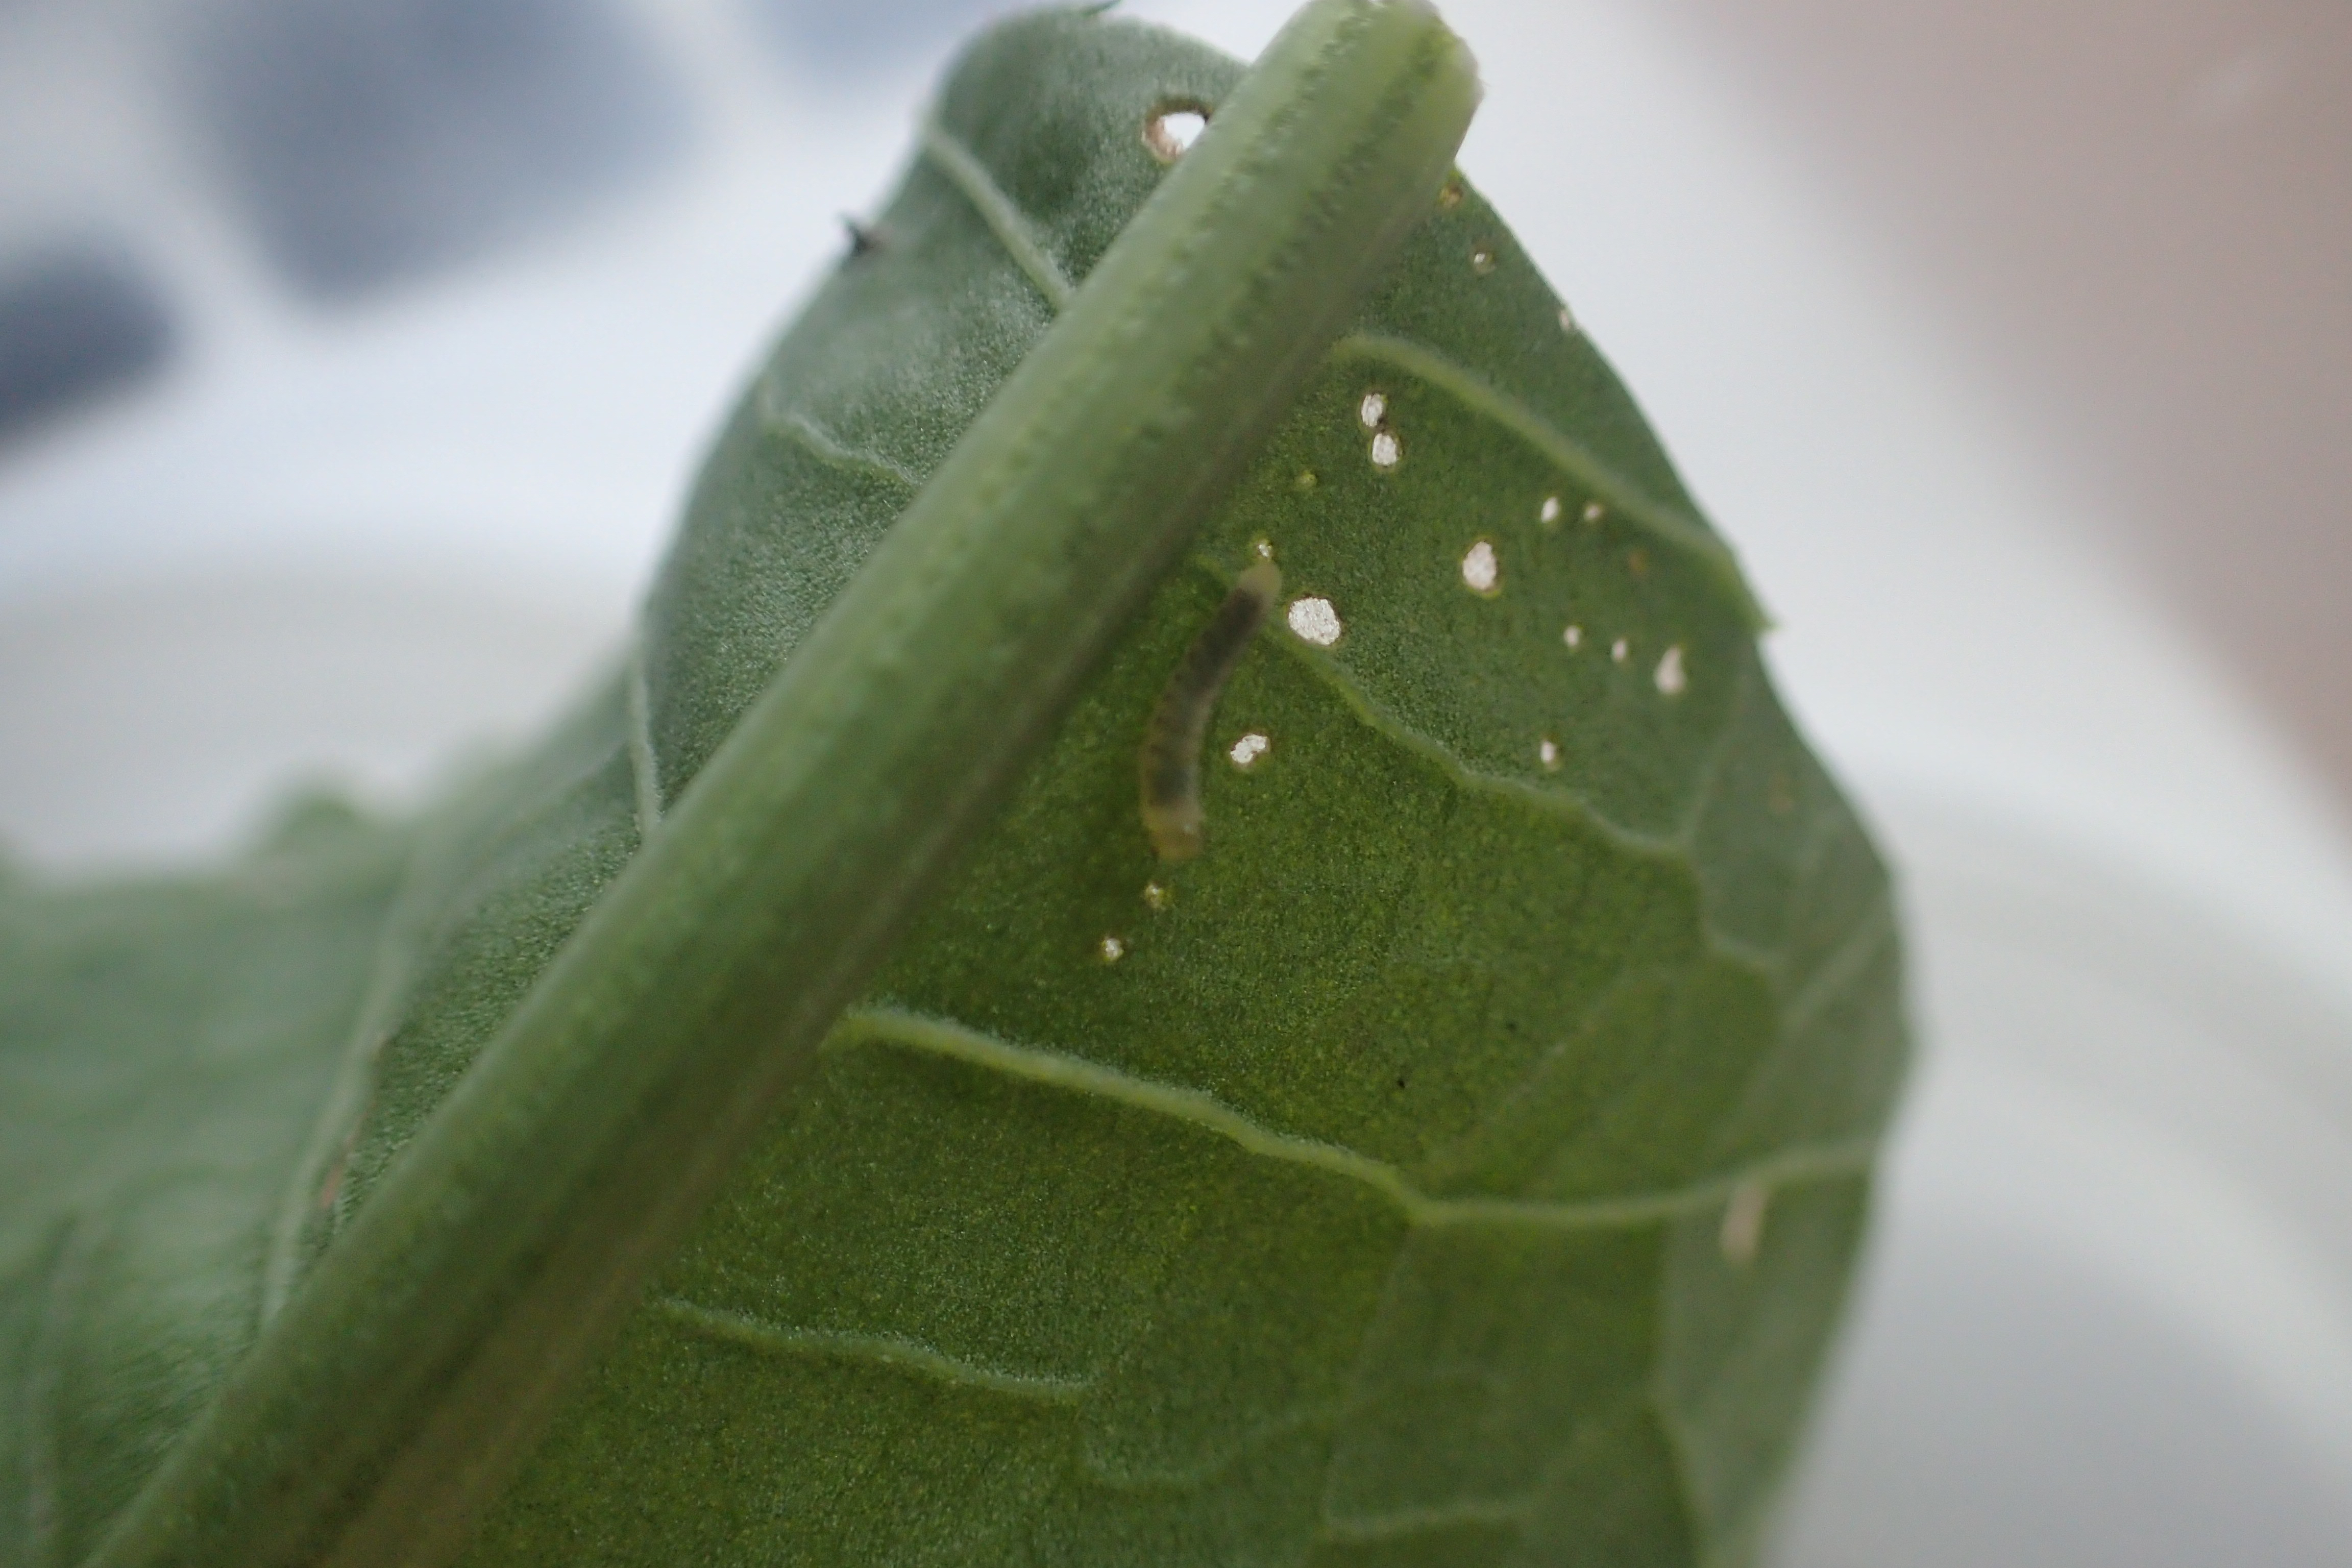
\includegraphics[width=5cm]{photo/hagurohabachi1.JPG}
    \caption{スイバの葉裏でよく見つかったハグロハバチと思われる幼虫}
    \label{pic-hagurohabachi}
  \end{center}
\end{figure}

そのまま, 公園の奥の方にスイバがまばらに生えている方に向かったところ, ほとんど葉がないスイバの, かなり上の方に, ぼてっとした幼虫が写真\ref{pic-sitting-on-branch}のように, とまっているのを発見. 
\begin{figure}[htbp]
  \begin{center}
    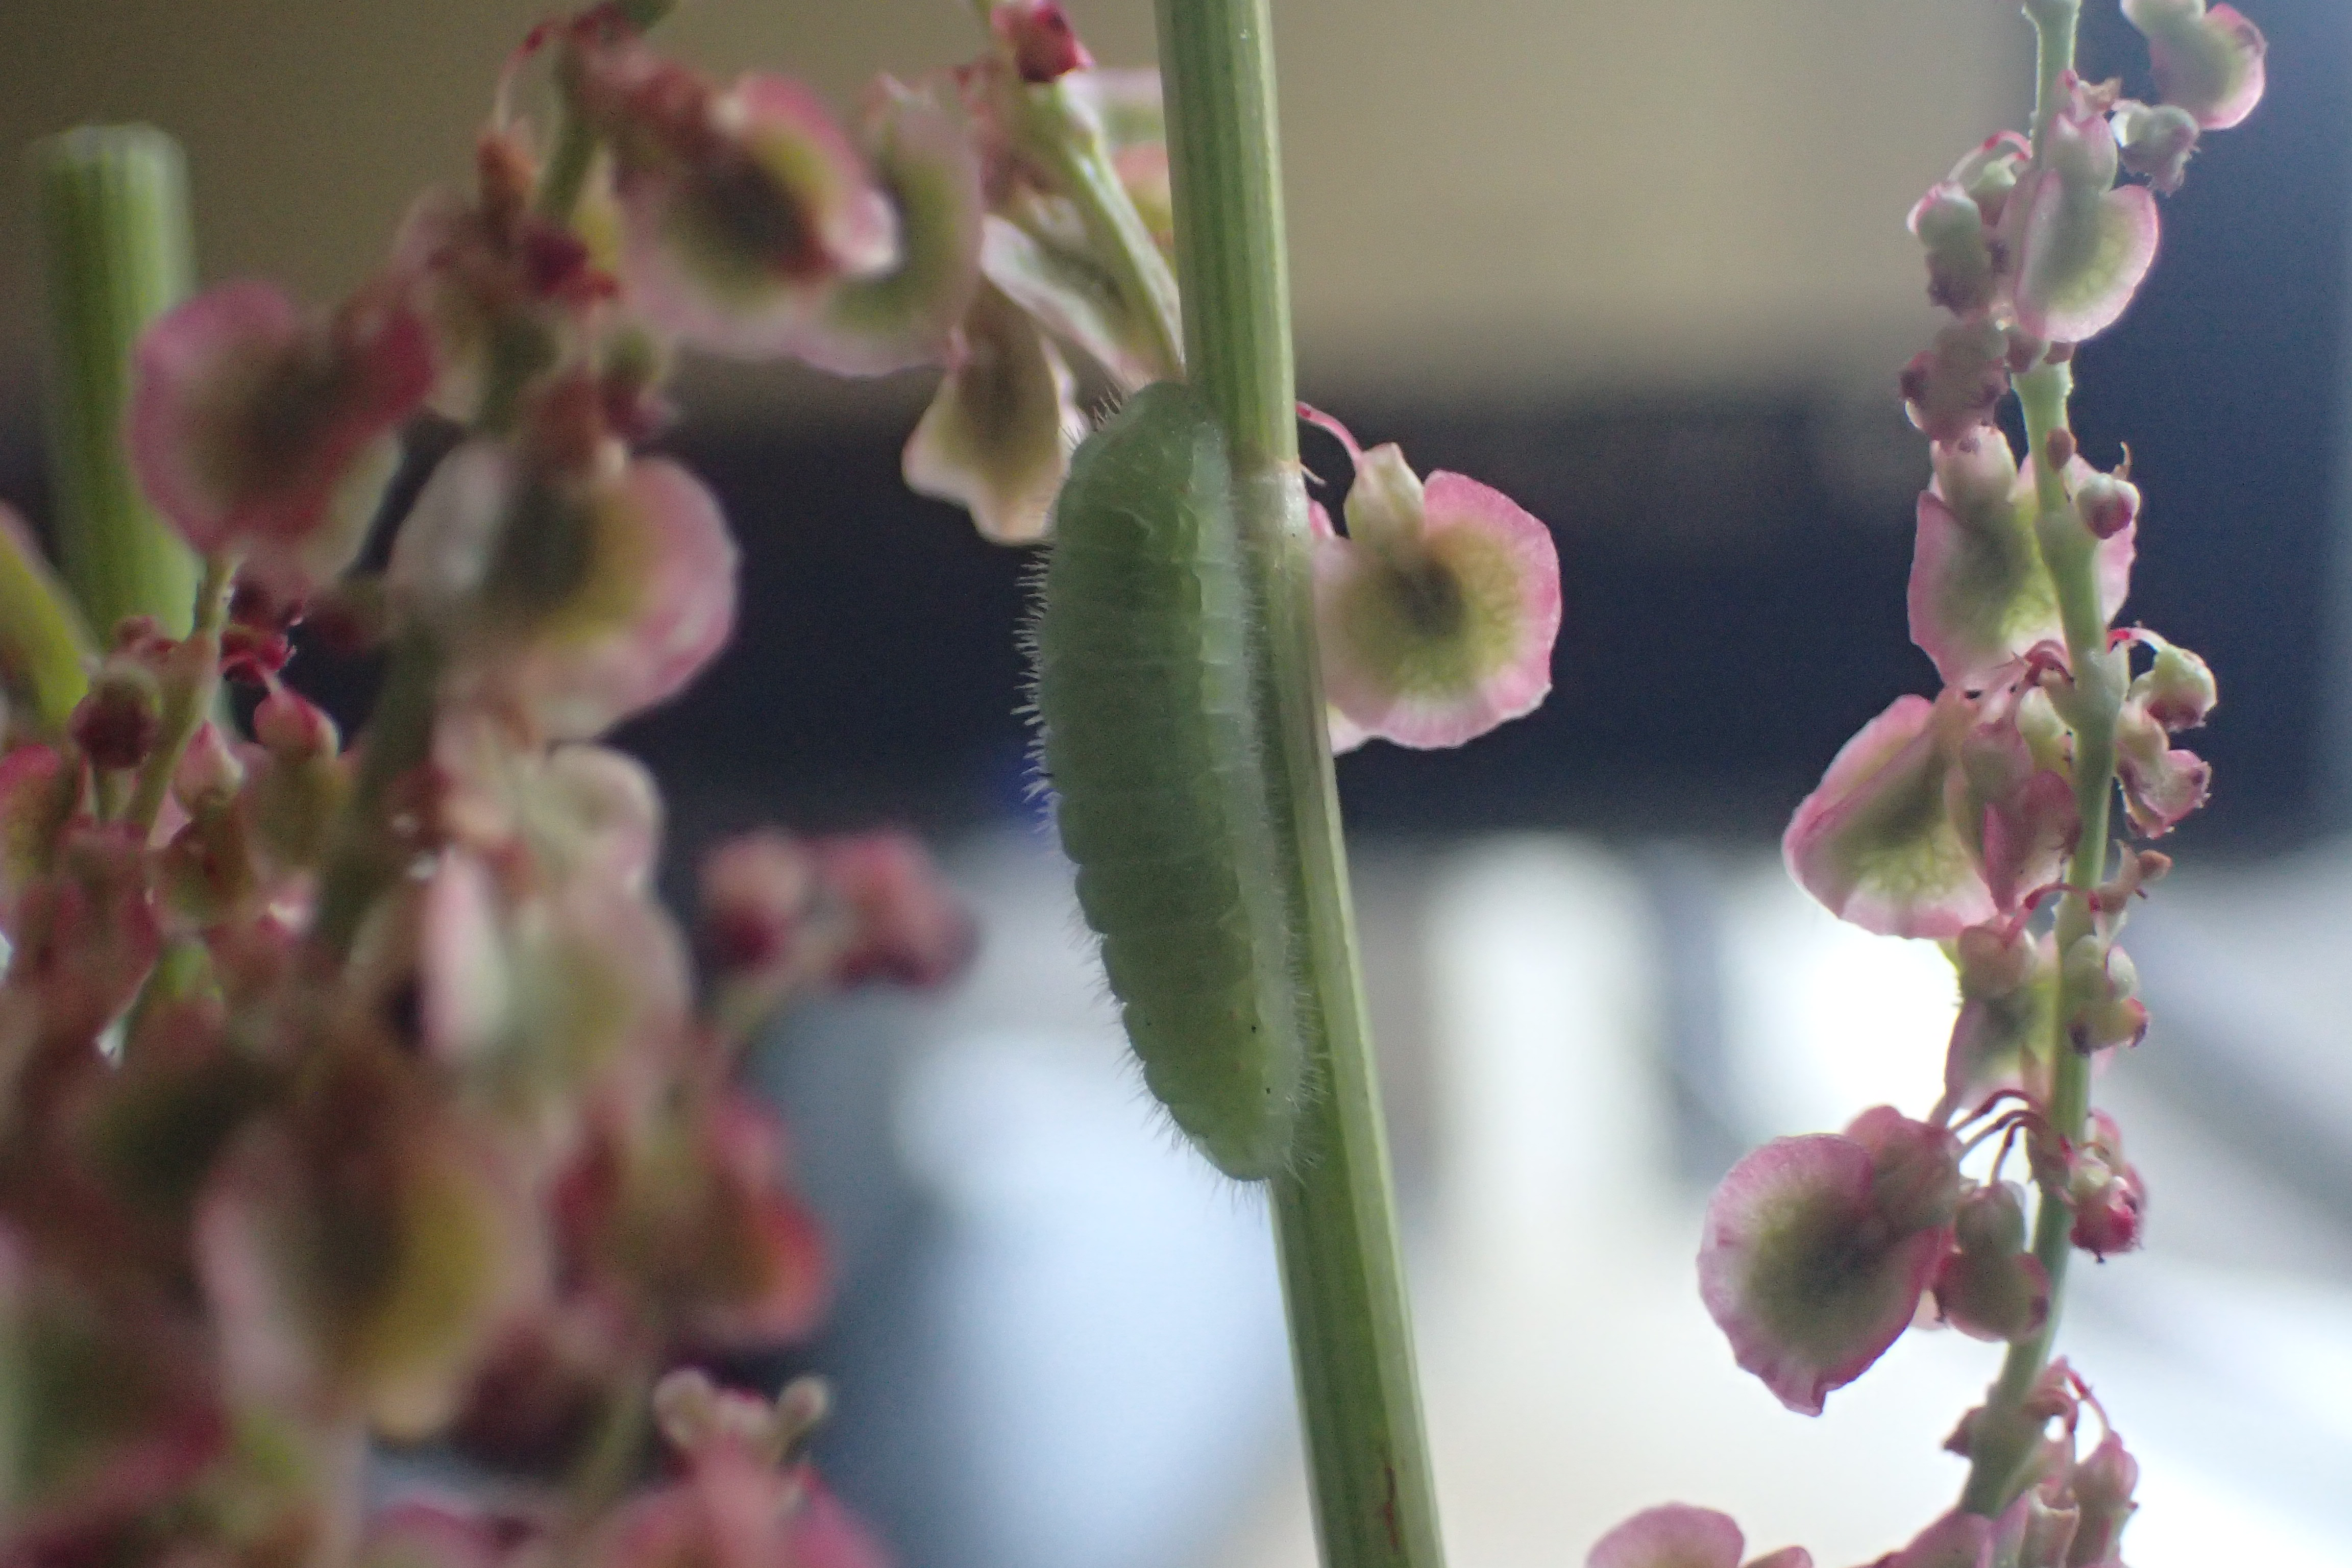
\includegraphics[width=5cm]{photo/sitting_on_branch.JPG}
    \caption{スイバの枝で静止していた幼虫}
    \label{pic-sitting-on-branch}
  \end{center}
\end{figure}

同様なポイントを探したところ, すぐ2匹目が見つかった. 
写真\ref{pic-field}のような, 割とひらけた場所であっさり見つかるようだ. 
最初に見つけた幼虫は, 1cm以上のサイズで, 2匹目の幼虫も, 1cm 弱のサイズで, どちらも終齢か, 4齢程度の幼虫と思われる. 
この時期は, 発生サイクル的に, 終齢が多い可能性がある. また, 終齢の幼虫は, 葉裏より, 花を食する可能性がある. 

\subsection{16時半:飼育環境の構築}
まずは, 採集時のスイバが乾燥しないように, 水を満たしたケースにさしたところ, そのわずかな振動で, 幼虫がぽろっと落ちた. 
その後, 幼虫は花によじ登ろうとしているように見えたが, 素直によじ登るというよりも, 頭を振りながら身をよじる動作をしていた. その動作のせいか, 登りかけては落ちるのを繰り返していた. 
脚で食草にしがみつく力は, アゲハ属の幼虫に比べると, 極端に弱いと推測される. 
また, それゆえに, 糸を吐き, 足場を作ろうとして, 妙な動作をしていたのではないかと推測される. 
\begin{figure}[htbp]
  \begin{center}
    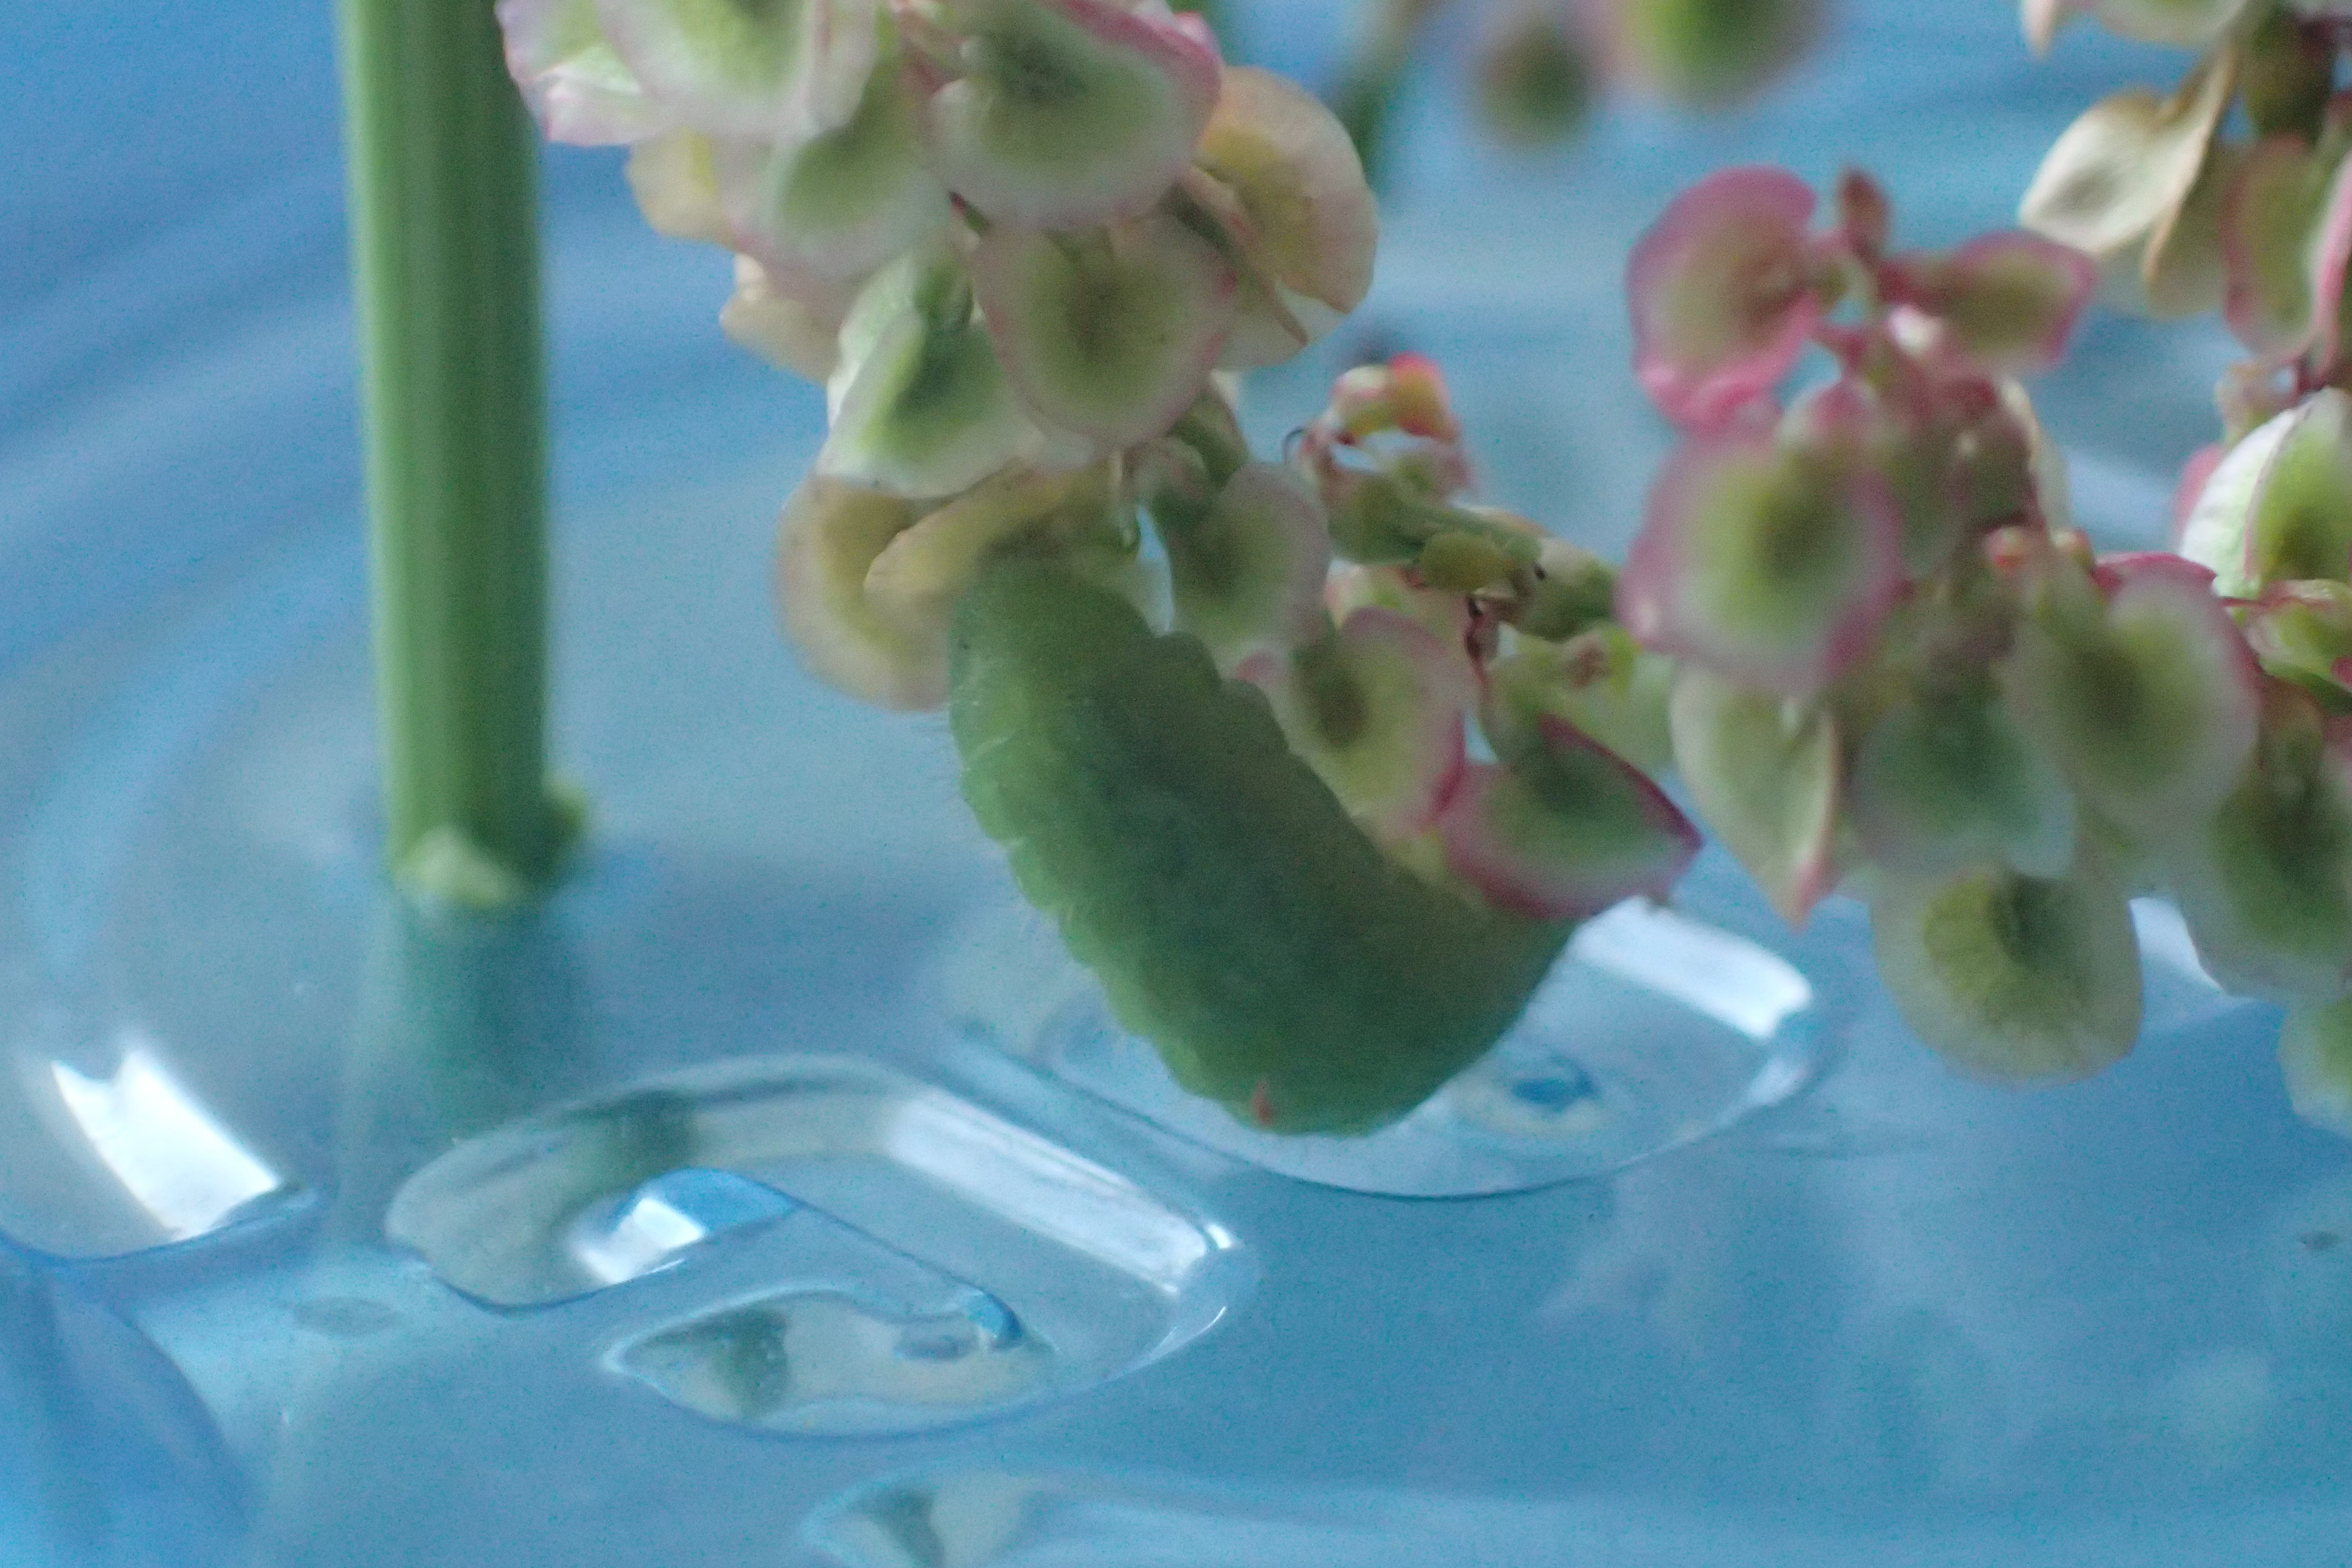
\includegraphics[width=5cm]{photo/try_to_climb.JPG}
    \caption{スイバの花によじ登ろうとする幼虫}
    \label{pic-try-to-climb}
  \end{center}
\end{figure}

\subsection{17時:飼育ケージの変更}
本来であれば, 自然界と同じように, スイバの花が垂直に上に伸びている状況を再現した方がよいと考えたが, 
枝から落下した幼虫があまりにも枝に戻ることができないのと, 世間のベニシジミ飼育のブログなどで, 枝を寝かせた状態で飼育しているものがほとんどであることから, 
枝を寝かせる方向にした. 捨てる予定であった, ガラスの耐熱ボウルを綺麗に洗浄し, スイバの枝に, 湿らせたキッチンペーパーを被せ, 
その上からアルミホイルでくるみ, 写真\ref{pic-environment}のような状況にした. 
\begin{figure}[htbp]
  \begin{center}
    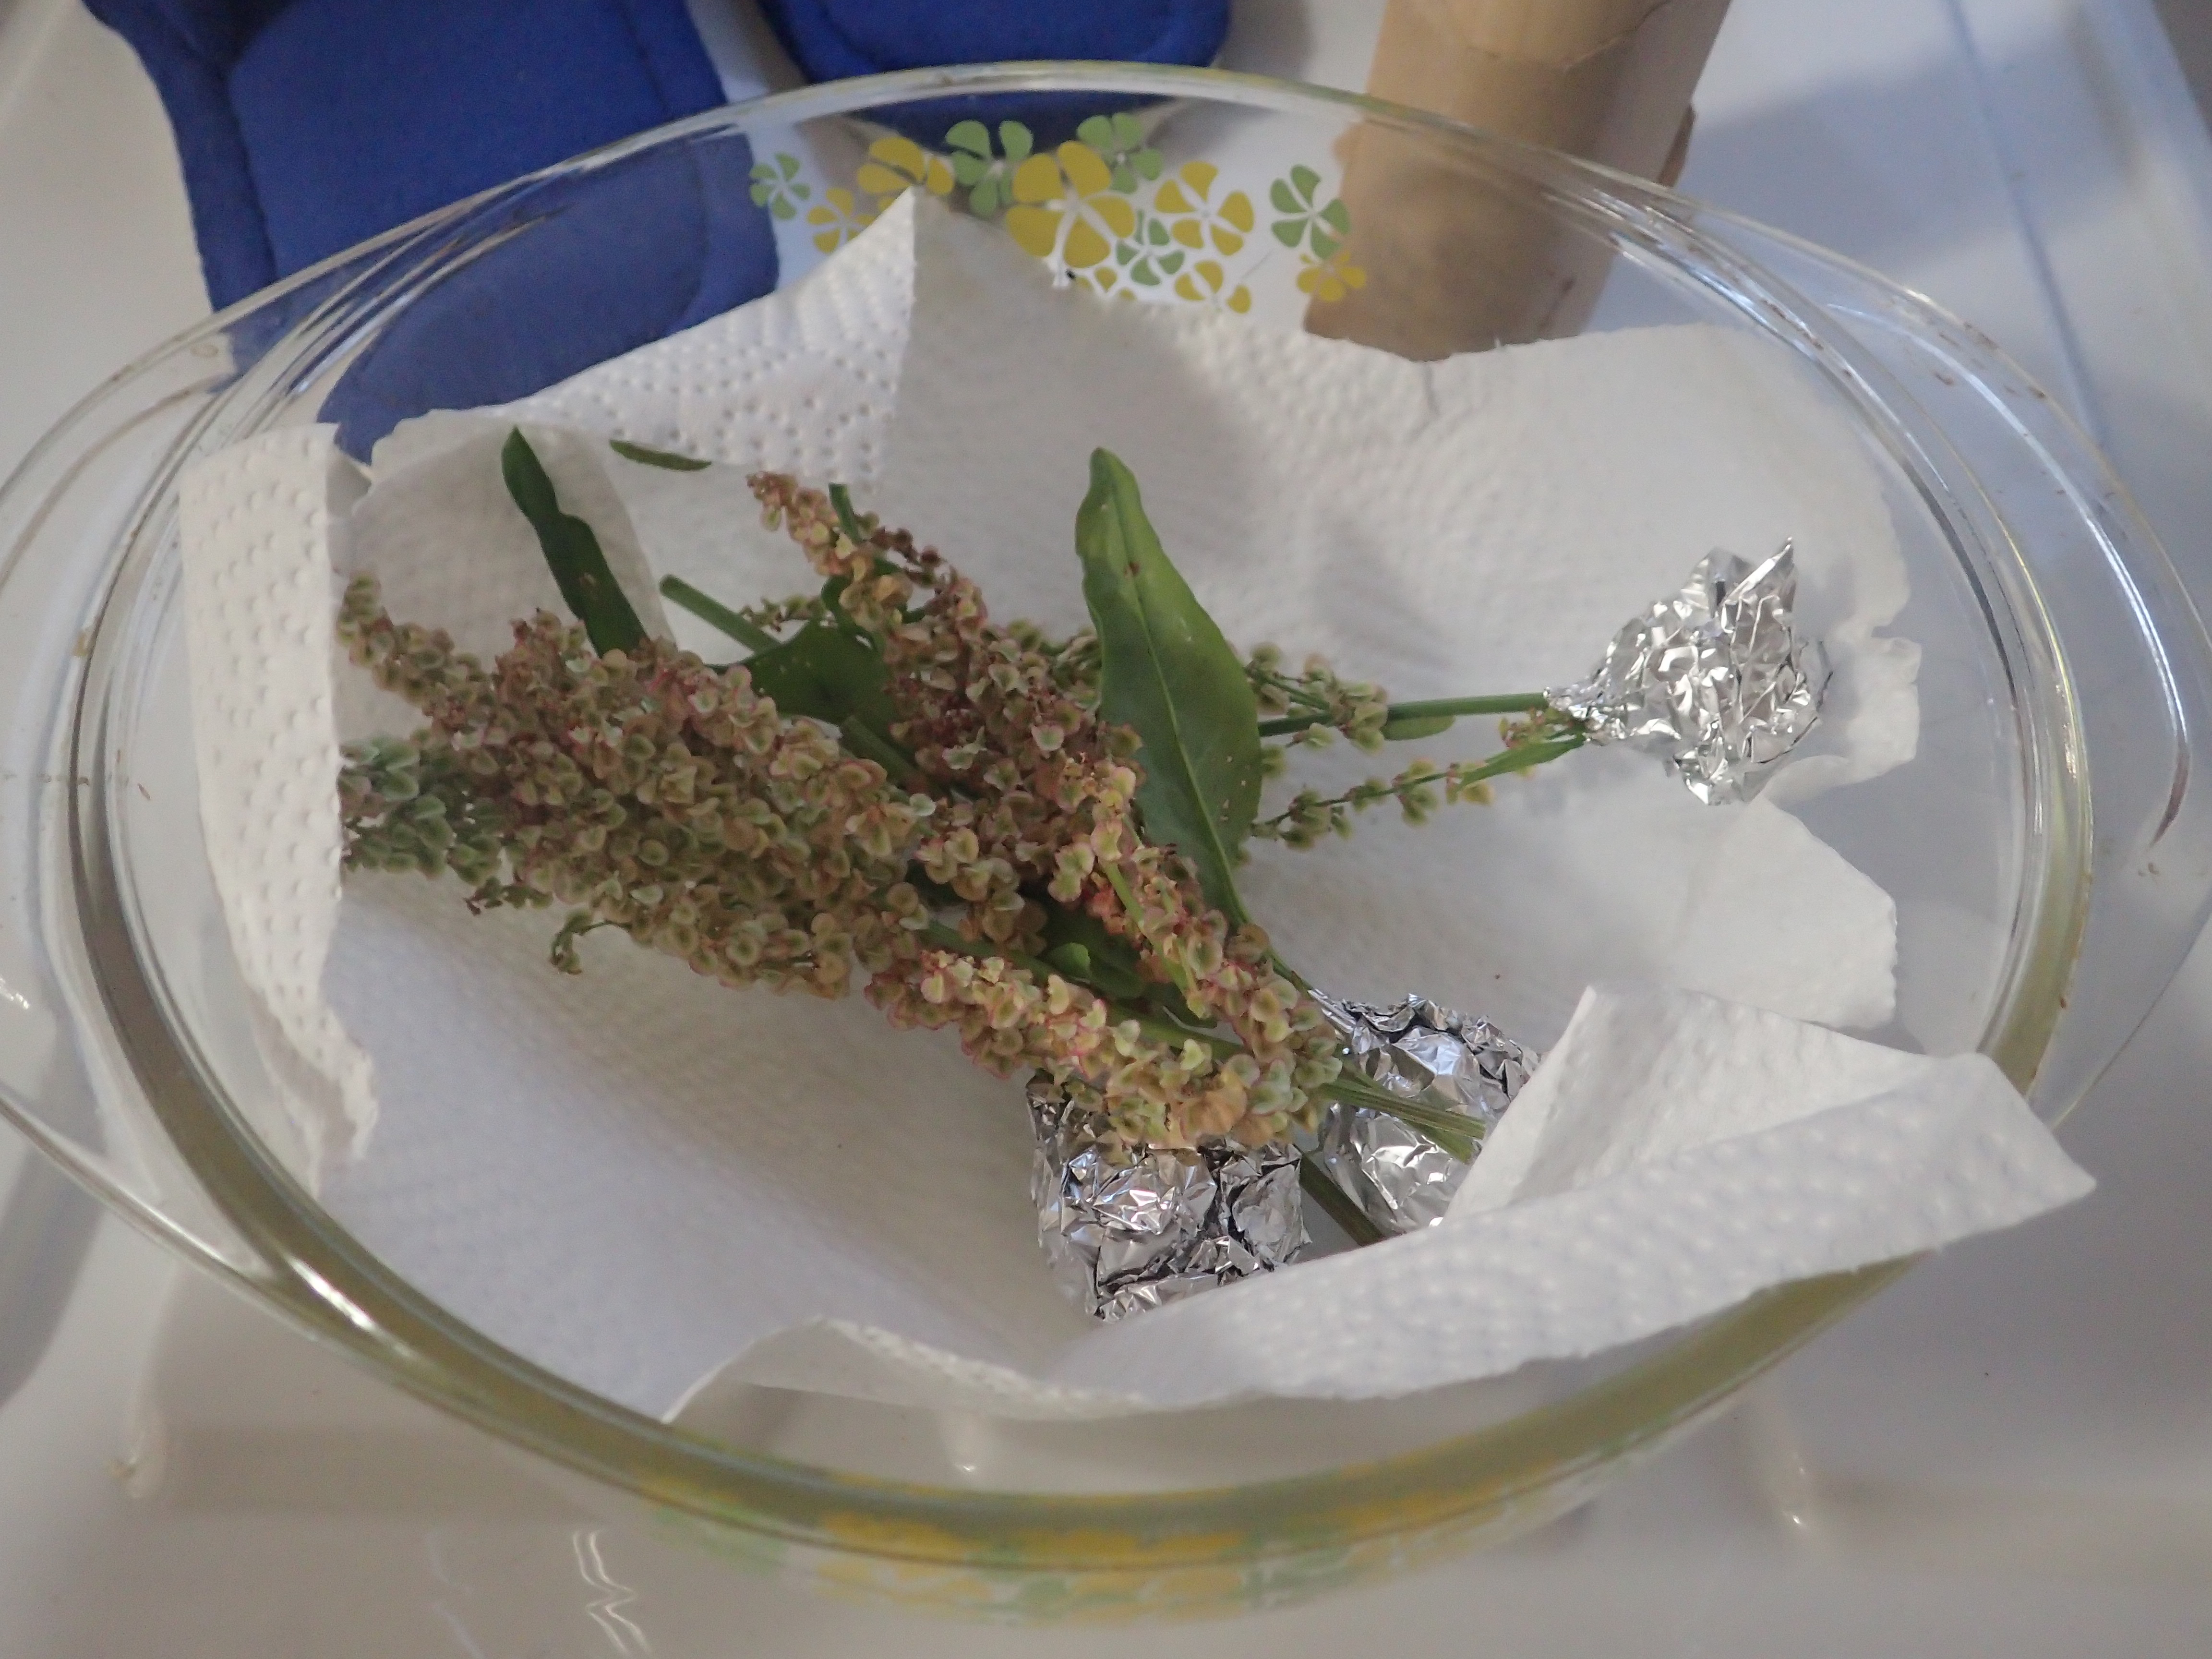
\includegraphics[width=5cm]{photo/environment.JPG}
    \caption{ガラスボウルによる飼育環境}
    \label{pic-environment}
  \end{center}
\end{figure}
また, ガラスボウルの底に, どうしてもスイバから漏れた水がたまり, 幼虫の溺死の危険があるため, 
底にはキッチンペーパーを敷いた. さすがの幼虫も, キッチンペーパーならば足が滑らないのか, 歩きやすそうに動いていた. 
その後, まだ外が少し明るかったので, 太陽光の代わりに, 爬虫類用のUVBランプに日没までの30分程度当てた. 
日本の環境にしては少し紫外線量が多いように思われたが, ガラス越しなので, 半減しているはずで, 問題はないと思われる. 

\subsection{18時:幼虫の移動}
食草の上を移動していた幼虫が, 2匹ともキッチンペーパーに降り, 移動を始めた. 
どこに移動するか見ていると, 写真\ref{pic-environment}の左上(よく見ると紙の裏から体がはみ出している)ように, やたらと紙の裏, 折れ曲がったところなどに移動して, そこで静止する様子が見られた. 
おそらく, 休む時は, 葉などの裏に隠れる習性からの行動であろうと思われる. 

\subsection{20時:活動の再開}
キッチンペーパーの裏でそのまま静止して翌朝まで寝てしまうのかと思ったが, 1時間程度しか静止しておらず, また移動し, 食草を食べている様子が確認できた. 
おそらく, 夜間でも, 短時間の休息と移動を繰り返すことで, 天敵に見つかる可能性を下げているのであろうと思われる. 
人間や, 犬猫と違い, 夜間にずっと寝ている, ということは無いようだ. 

\subsection{23時:糞の観察}
糞は, やや明るめの焦げ茶色で, 1mm程度の樽型のものが10個ほど確認できた. 

\newpage
\section{5/12の記録}
\subsection{9時:特に異常なし}
思いの外大量の糞をしていたので, 古い食草を捨てるとともに, 掃除. 
昨日, 枝に登るのに苦労していた個体も, しっかり枝に捕まって静止していた. 
寸法を測定したところ, どちらも15mm*5mm程度で, 思ったより寸法差はなかった. 
葉が食われていたが, 表面だけを舐めるような食痕ではなく, 写真\ref{Larba-day2-2}のように, アゲハのような食痕であった. 
他のブログなどと矛盾するが, 与えている葉が, 柔らかい若い葉であることが要因なのかもしれない. 

\begin{figure}[htbp]
  \begin{minipage}{0.5\hsize}
    \begin{center}
      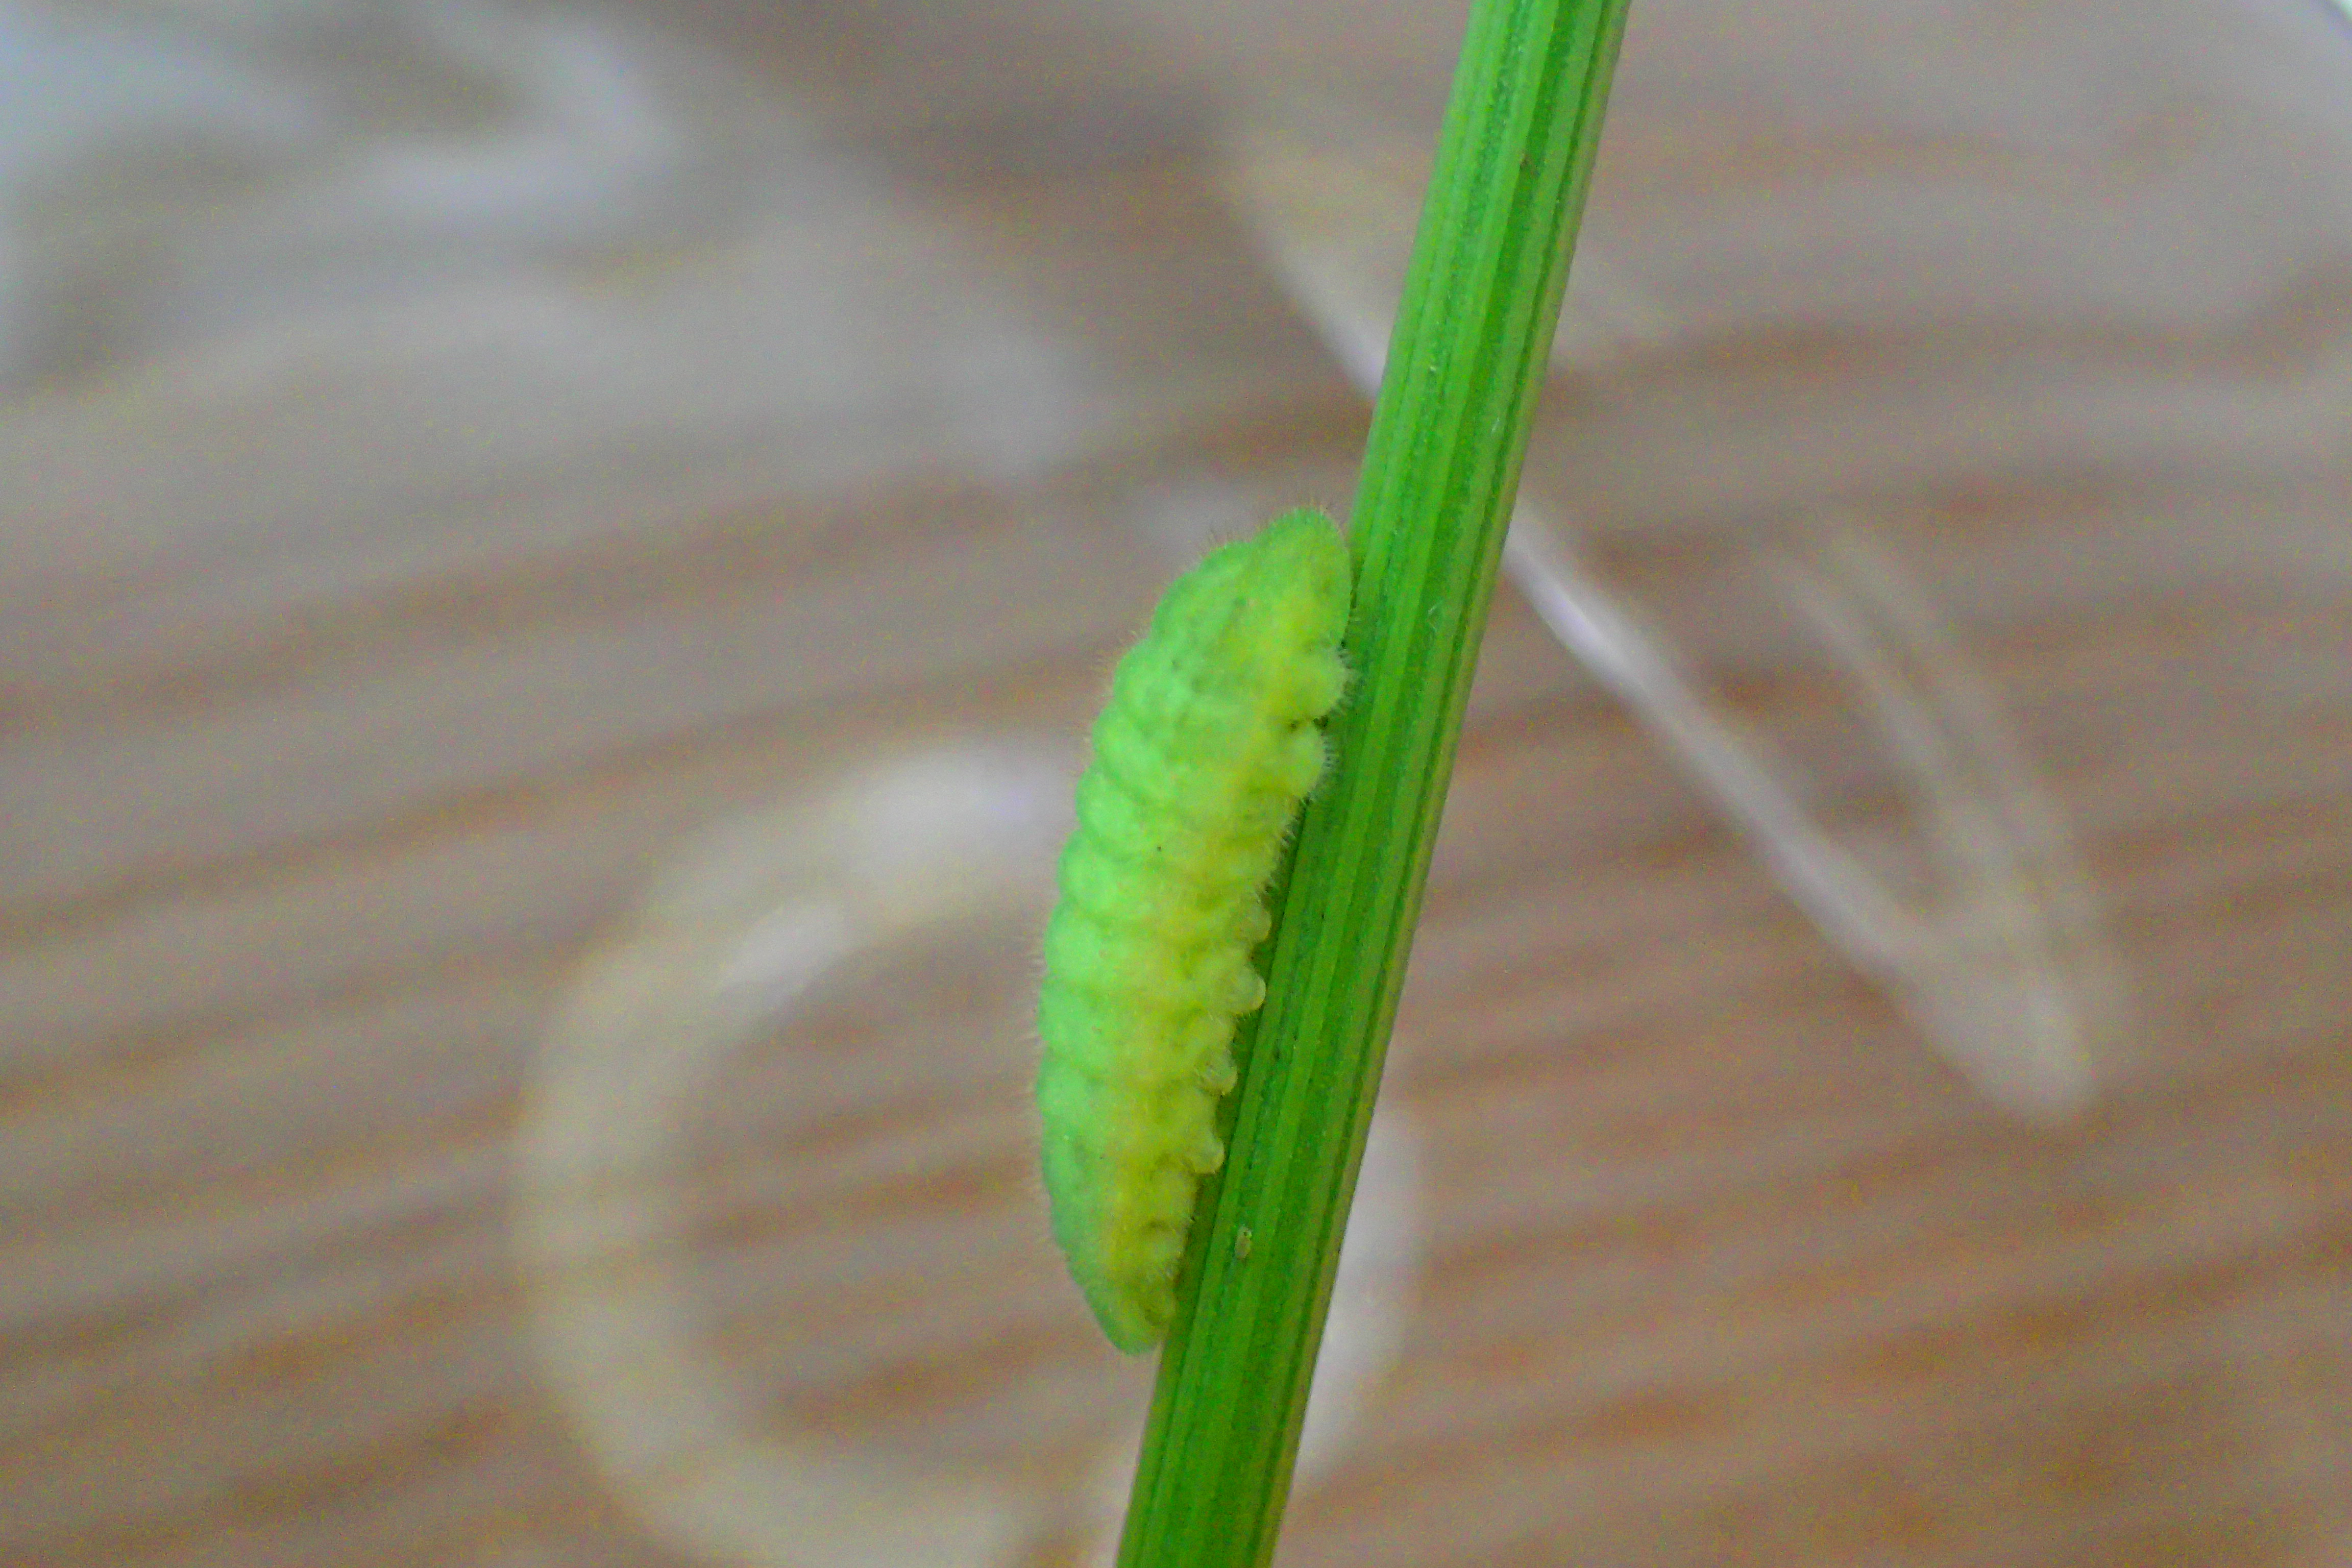
\includegraphics[width=5cm]{photo2/Larva1.JPG}
    \end{center}
    \caption{幼虫1の状態}
    \label{Larba-day2-1}
  \end{minipage}
  \begin{minipage}{0.5\hsize}
    \begin{center}
      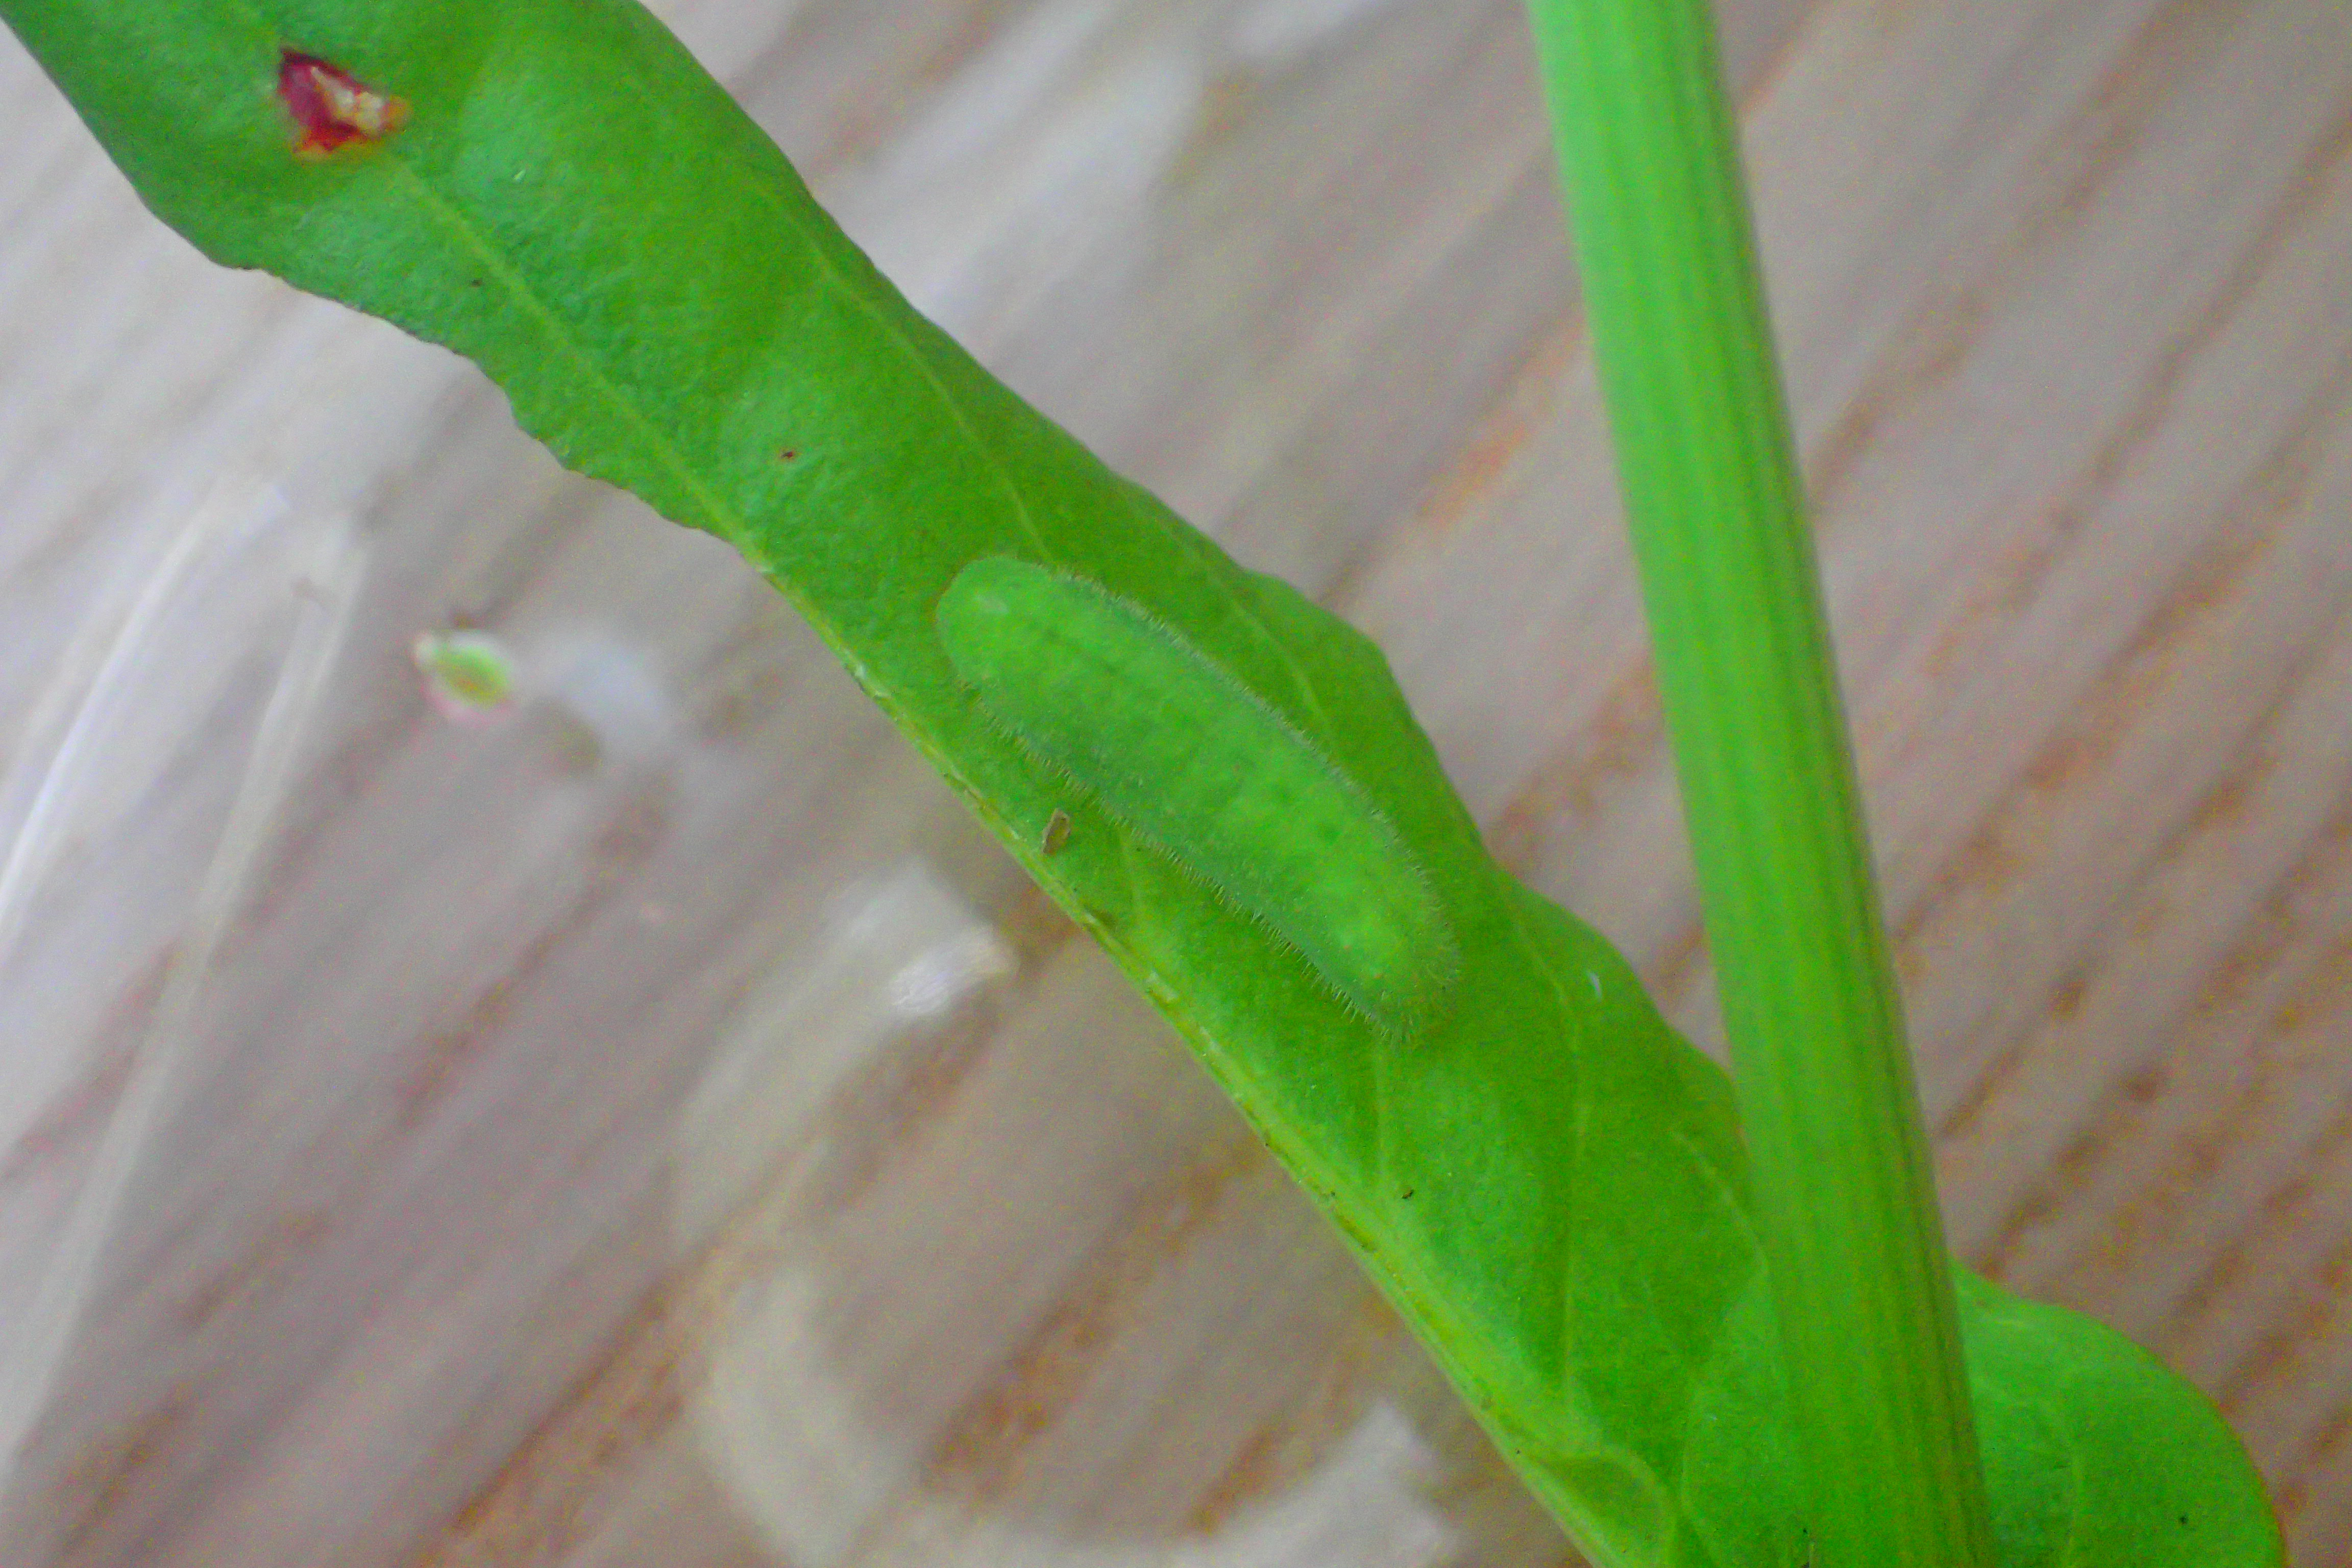
\includegraphics[width=5cm]{photo2/Larva2.JPG}
    \end{center}
    \caption{幼虫2の状態}
    \label{Larba-day2-2}
  \end{minipage}
\end{figure}

\subsection{15時:餌の採取と幼虫の居場所}
幼虫の採集場所と同じところに, 新しい餌用のスイバを取りに行ったついでに, 
幼虫を探した. 簡単に, 同じ苗で2匹見つかったが, やはりどちらも, 花に近いところの枝, 花の中で見つかった. 
やはり, 幼虫はあまり葉にいないのだろうか. 
家に帰り, ケージ内の幼虫がどこにいるか見たところ, 2匹とも花を避け, 葉の上にべったりとくっついていた. 
単純に花, 葉というより, 鉛直方向に上を目指す傾向があるだけなのか. 
よくわからない. 


\end{document}
